\begin{figure}
\centering
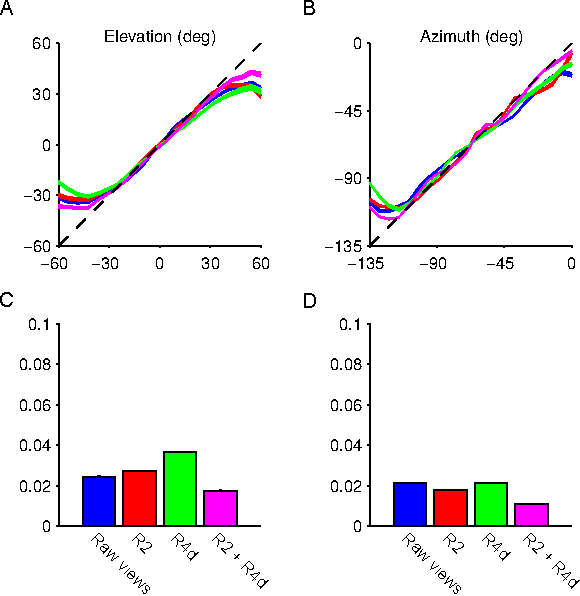
\includegraphics{figures/elaz}
\caption{Performance of neural networks trained using different visual information as inputs.
Separate neural networks were used for raw views (36~pixels), R2 neurons ($N=28$), R4d neurons ($N=14$), and R2 and R4 neurons ($N=42$).
The networks were trained simultaneously to discriminate elevation and azimuth, both of which were normalised to be between 0 and 1.
A--B: The network activation for the four different neural networks in response to a range of different elevations/azimuths.
The error bars indicate standard error.
C--D: The mutual information between stimuli and responses, $I(\mathcal{S},\mathcal{R})$, for the four different types of input to the network, for a range of elevations/azimuths.
}
\label{fig:elaz}
\end{figure}
